\documentclass[12pt]{article}
\pagestyle{plain}
\linespread{2}

% Document
\title{HDMI Divider}
\author{Cassandra Chow}

% Declarations
\usepackage{graphicx}
\DeclareGraphicsExtensions{.jpg}

\frenchspacing
\usepackage{indentfirst}
\usepackage{fullpage}
\usepackage{float}

\begin{document}
\maketitle

% ABSTRACT
\begin{abstract}
With the detailed project we will strive to design an embedded system that will enable the user to divide a primary high-definition multimedia interface (HDMI) display source into two separate outputs that each display half of the primary display. The application of this device if focused at enabling video game players to assign parts of the game display to other dedicated displays which can be useful for multiplayer games designed with split-screen gameplay. To do this, our product will need to accept HDMI input frames, divide that input into two separate output frames, and process the output frame to suit their individual displays. 
\end{abstract}

\pagebreak
\tableofcontents

% INTRODUCTION
\pagebreak
\section{Introduction}

Our product, which we will call an HDMI Divider for now, will be designed to give its user a solution to dividing split-screens that is not otherwise offered by the application or display hardware itself. The application of the HDMI splitter is illustrated in Figure~\ref{fig:concept}. Because the HDMI divider will be able to accept HDMI signals from an arbitrary source device, it's application can be utilized across any platform using HDMI output. Giving consumers the option of dividing their display can enhance the experience of video game players especially in competitive gameplay. Where players are competing, it is in the best interest of each user to win against the other in some manner but a split-screen setup prevents the players from concealing their actions from the other. Another reason players might find this device attractive is just the ability to expand their split portion of the screen to a larger display.

\begin{figure}[H]
\centering
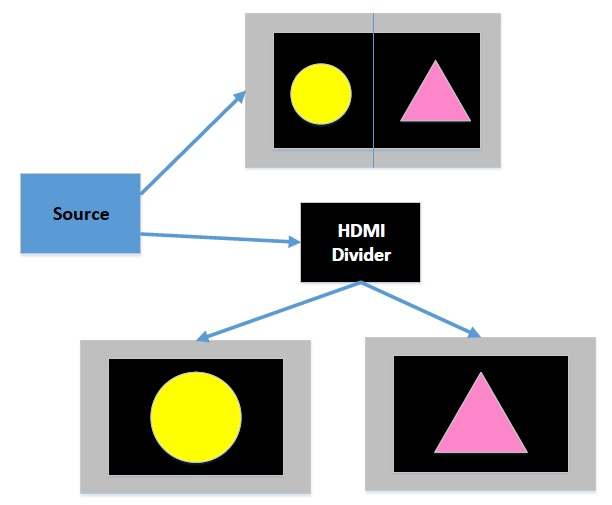
\includegraphics[width=0.9\textwidth]{Concept.jpg}
\caption{Represents use model concept of the HDMI divider dividing a split-screen into two dedicated displays}
\label{fig:concept}
\end{figure}

This project also acts as a challenging learning experience to an undergraduate student. Since we will be utilizing the digital logic on a field-programmable gate array (FPGA) to accomplish our device implementation, we will not only become more familiar with FPGA applications but also obtain a better grasp on embedded system architecture and the HDMI protocol specification. Most projects of interest to us required in-depth knowledge in protocols that are widely used in various electronics, therefore a project which includes development on the HDMI is the main reason for undertaking this task. All of the above benefits will be sought out in order to improve our design capabilities as an engineer. 

% METHODS, TECHNIQUES, and DESIGN
\section{Methods, Techniques, and Design}

% DESIGN CONSIDERATIONS
\subsection{Design Considerations}

To understand the requirements for our project we must examine our resource requirments which includes knowing what data we are acquiring, how the data is being acquired, and what our device will do with that data. For our application model we will require the display data from some external source which will be transmitted via the HDMI interface. The received display data must be processed and then output across two individual displays. Our target display format is the standard HDTV configuration which supports a resolution of 1920x1080p. The platform we decided on to implement our design is an FPGA. FPGAs are known for being able to perform signal processing quickly which is critical in display applications. The specific development platform we will be using is Altera's DE2-115 Development and Education board.The DE2 provides us with sufficient means in accomplishing our project requirements while also being flexible to future changes.

% HDMI DISPLAY
\subsection{HDMI Display}

According to the HDMI specification, there are three data channels used to transmit pixel data typically at a resolution of 24 bits per pixel, 8 bits per channel. The HDMI interface has a pixel clock that functions at a maximum of 165 MHz \cite{Ref_HDMI_Spec}. The DE2 can support the necessary switching speed on it's I/O lines but the on-board SRAM and SDRAM have insufficient bandwidth capabilities to store the data fast enough. We will therefore be writing to the embedded memory on the FPGA chip allowing us to take advantage of the speed capabilities on the FPGA. There are only 486 Kbytes of embedded memory on the Cyclone IV DE2 FPGA chip \cite{Ref_Memory_Block}, so we cannot store entire frames but this is sufficient space to store the each line of data for each input and output frame until it it is processed. Then by using a simple image rescaling algorithm, such as nearest neighbor or interpolation, we can als ensure we are able to resize the image properly even if we cannot send and receive an entire frame at once.

There is no onboard solution for implementing the HDMI protocol on the DE2 board, therefore we will being using HDMI transmitter and HDMI receiver chipsets. Each selected chipset requires approximately 32 I/O lines \cite{Ref_HDMI_Rx} to interface with the DE2 but the DE2 board only has 36 GPIO pins mapped to the the Cyclone IV \cite{Ref_DE2}. However, we can expand the number of GPIO pins available by connection an expansion board to the DE2's High-Speed Mezzanine Connector (HSMC), giving us access to another three GPIO headers. Since we only need 3 HDMI interface, 1 input and 2 outputs, we will only have enough GPIO pins available if we use the HSMC GPIO expansion daughter card. To implement the HDMI chipsets and connection, we'll be designing a PCB for each to interface with the DE2 though the GPIO expansion. Our implementation for our device is illustrated by the system block diagram in Figure~\ref{fig:block}.

\pagebreak

% BLOCK DIAGRAM
\subsection{System Block Diagram}

\begin{figure}[H]
\centering
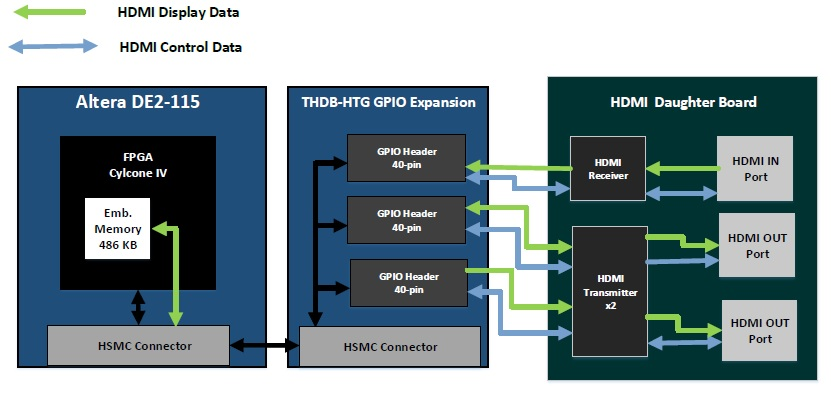
\includegraphics[width=0.9\textwidth]{Block_Diagram_v2.jpg}
\caption{Block Diagram of device implementation}
\label{fig:block}
\end{figure}

\pagebreak

% PARTS LIST
\section{Parts List}

These are the primary components required for our HDMI Divider implementation

\begin{itemize}
\item Altera DE2-115 Education and Development Board \cite{Ref_DE2}
\item THDB-HTG GPIO daughter board \cite{Ref_GPIO_daughter}
\item ADV7611 HDMI Receiver \cite{Ref_HDMI_Rx}
\item AD9389B HDMI Transmitter x2 \cite{Ref_HDMI_Tx}
\end{itemize}

% TIMELINE
\section{Timeline}

Figure~\ref{fig:timeline} is the task timeline we have set for ourselves over the next 12 weeks of development. By the end of 12 weeks we should be able to confirm HDMI input and output functionality including the memory architecture requirements. Notice that we are not going to be working on the image processing required for dividing and resizing the display output yet, just establishing the protocol functionality on the FPGA.

\begin{figure}[H]
\centering
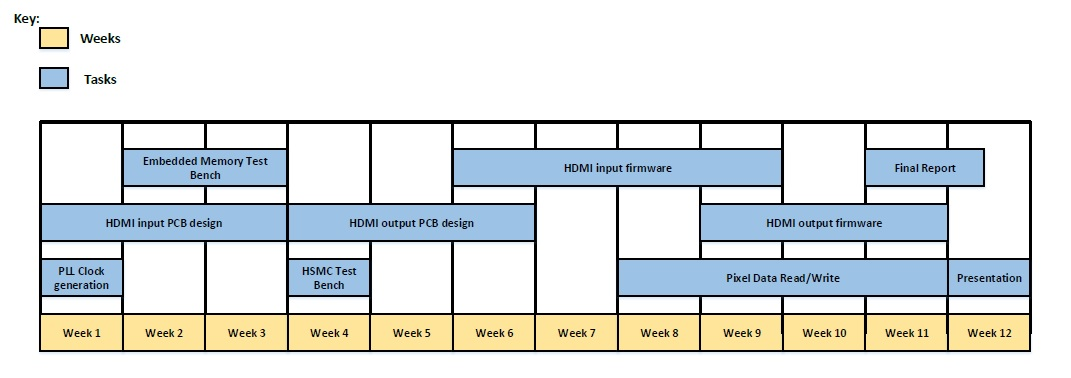
\includegraphics[width=0.9\textwidth]{Timeline.jpg}
\caption{Timeline for development tasks}
\label{fig:timeline}
\end{figure}

\begin{description}
\item[PLL Clock Generation] Configuring the PLL on the FPGA to generate desired clock rates for processing
\item[HDMI Input PCB Design] Designing the PCB for the daughter card implementing the HDMI input port and interface
\item[HDMI Output PCB Design] Designing the PCB for the daughter card implementing the HDMI output port and interface
\item[Embedded Memory Test Bench] Configuring embedded memory system and testing read/write functionality
\item[HSMC Signal Test Bench] Configuring signal I/O over the HSMC to GPIO bus and testing functionality
\item[HDMI Input Firmware] Developing FPGA digital logic for receiving HDMI display data
\item[HDMI Output Firmware] Developing FPGA digital logic for transmitting HDMI display data
\item[Pixel Data Read/Write] Developing the read/write process for storing display data in memory
\item[Final Report] Compiling final project results into a report document
\item[Presentation] Preparing and delivering presentation of project results
\end{description}

\section{Citation}
\bibliographystyle{plain}
\bibliography{Citation}

\end{document}

